\documentclass[12pt,a4paper]{article}
\usepackage[polish]{babel}
\usepackage[T1]{fontenc}
\usepackage[utf8x]{inputenc}
\usepackage{hyperref}
\usepackage{url}
\usepackage{graphicx}
\usepackage{listings}
\usepackage{amsmath}
\usepackage{indentfirst}
\usepackage[]{algorithm2e}
\addtolength{\hoffset}{-1.5cm}
\addtolength{\marginparwidth}{-1.5cm}
\addtolength{\textwidth}{3cm}
\addtolength{\voffset}{-1cm}
\addtolength{\textheight}{2.5cm}
\setlength{\topmargin}{0cm}
\setlength{\headheight}{0cm}
\lstset{
  breaklines=true
}
\begin{document}
	
	\title{Dokumentacja projektu\\ Języki Skryptowe}
	\author{Adam Kieart, gr. 2C, semestr III}
	\date{\today}
	
	\maketitle
	\newpage
	\section*{Część I}
	\subsection*{Opis programu}
	 Projekt ma za zadanie przekształcanie dat zapisanych w postaci binarnej na zapis dziesiątkowy w formacie [rok-miesiac-dzien]. Projekt zawiera skrypt napisany w języku Batch. Po wykonaniu wszystkich operacji zawartych wyświetla dane na generowanej stronie internetowej.
	 \\
	\\ 	
    \textbf{Treść zadania z serwisu SPOJ.com :}
    \\ 	
    Różnych sposobów zapisu daty i czasu (o czym wielokrotnie się wszyscy przekonywaliśmy) jest całe mnóstwo i nierzadko z tego powodu można popaść z zupełnie niespodziewane kłopoty. Weźmy pod uwagę choćby taki aspekt problemu – Polacy zwykli zapisywać daty w naturalnej dla nich kolejności DD.MM.RR (w tej konwencji zapis 01.05.09 oznacza pierwszy maja roku 2009). Amerykanie czynią to zupełnie inaczej, stosując formę MM.DD.RR (a więc ten sam zapis dla Amerykanina oznaczać będzie piąty stycznia). Międzynarodowa norma ISO 8601 zaleca, aby daty (niezależnie od zwyczajów i konwencji lokalnych) zapisywać w konwencji RRRR-MM-DD i takiego też sposobu będziemy używać w naszym zadaniu.

Systemy komputerowe mogą wprowadzać jeszcze bardziej skomplikowane konwencje, służące np. minimalizacji rozmiaru pamięci potrzebnej do przechowywania daty.

Przyjrzyjmy się bliżej sposobowi (nazwijmy go roboczo standardem DOSFAT), w jaki poczciwy system DOS z systemem plików FAT przechowuje datę modyfikacji pliku. Używa się do tego celu jedynie szesnastu bitów i czyni się to w sposób następujący:

 
\begin{itemize}
\item   pierwszych 7 bitów koduje liczbę lat począwszy od roku 1980 (oczywistym jest, że pomysłodawcy tego rozwiązania nie przewidywali konieczności pamiętania dat sprzed tego roku, ale musieli zapewne domyślać się, że po roku 2107 cały ten wynalazek stanie się bezużyteczny)
\end{itemize}
\begin{itemize}
\item  kolejne 4 bity kodują numer miesiąca (tu nie ma niespodzianek – 0001 to styczeń, a 1100 to grudzień
\end{itemize}
\begin{itemize}
\item  ostatnie 5 bitów to numer dnia miesiąca (tu również nie natkniemy się cokolwiek niespodziewanego)
\end{itemize}

	 \\
	\\ 	
  \textbf{Polecenie }: napisz program, który wczyta ze standardowego wejścia datę zapisaną w konwencji DOSFAT (ciąg 16 cyfr binarnych) wypisze odpowiadającą jej datę zapisaną w konwencji przeciwnej. 
	 

	\newpage\newpage
	\subsection*{Instrukcja obsługi}
	Aby rozpocząć działanie programu należy uruchomić plik wykonywalny start.bat. W menu wyboru wybrać odpowiednią opcję.
    
\begin{enumerate}
\item Rozpoczęcie działania całego programu.
\item Wyświetlanie informacji o projekcie.
\item Wykonanie kopii zapasowej
\item Wyjście z programu
\end{enumerate}
	
Poniżej znajduje się zrzut ekranu z zaznaczonym plikiem startowym.
		
			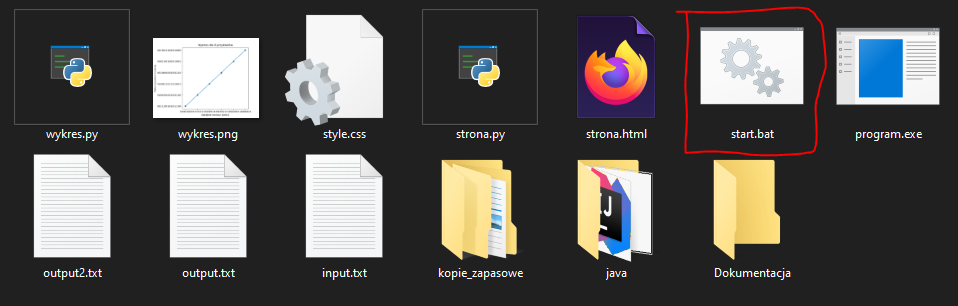
\includegraphics[scale=0.65]{instrukcja}
             	 \\
         	\\
			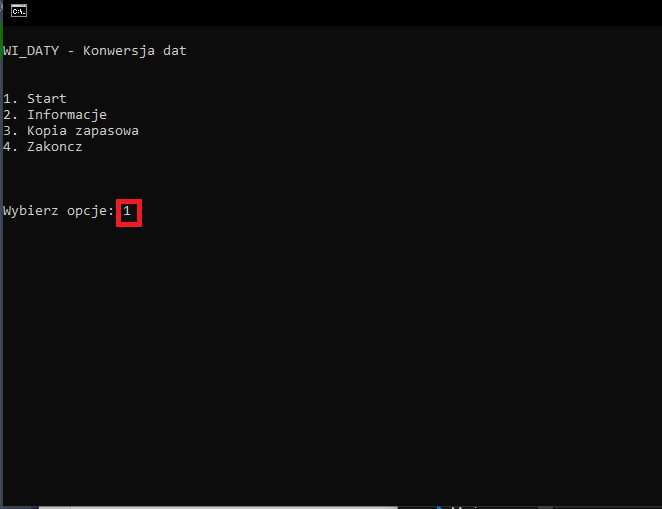
\includegraphics[scale=0.8]{instrukcja2}

		
	
	
\newpage
	\section*{Część II}
	\subsection*{Część techniczna}
\\
\\
Cały projekt obsługiwany za pomocą pliku start.bat. Skrypt pozwala nam na zarządzanie całym programem. Pozwala na rozpoczęcie pracy programu, wyświetlenie informacji o projekcie, wykonanie kopii zapasowej. Po wybraniu opcji numer 1 (Start) skrypt uruchamia program.exe, który wykonuje operacje konwersji dat. Następnie sprawdza, czy w folderze wykonywalnym istnieje wygenerowany wykres. Jeśli plik wykres.jpg nie istnieje, to zostaje uruchomiony skrypt o nazwie wykres.py, który genereuje wykres z pliku output2.txt. Do poprawnego działania skryptu generującego wykres niezbędna jest bibiloteka matplotlib
\\
\\
Program.exe, został napisany w języku Java, wygenerowany do pliku .jar następnie został skonwertowany za pomocą programu Launch4j do rozszerzenia .exe. Program.exe pobiera plik o nazwie input.txt, z którego czyta linia po linii daty zapisane w postaci binarnej. Kolejnym krokiem jest konwersja pobranych danych na system dziesiętny oraz zapis do dwóch osobnych plików (output.txt,output2.txt)
\\
\\
Jeśli operację wykonywane przez program.exe powiodą się, zostaje uruchomiony skrypt strona.py. Skrypt ten napisany w języku Python.. Skrypt ma za zadanie wygenerowanie pliku strona.html, który pokazuje rezultaty pracy pliku program.exe. Pobiera dane z plików (input.txt,output.txt) i przedstawia je w postaci czytelnej tabelki. Poniżej tabelki jest wyświetlany plik wykres.jpg. Do poprawnego działania wymagana jest biblioteka glob.
\\
\\
Ostatecznie program.exe uruchamia plik strona.html wygenerowany w poprzednim kroku. Skutkuje to otwarciem przeglądarki i prezentacją danych. Stylizacja pliku strona.html jest zarządzana z pomocą pliku styl.css


	\newpage
	\subsection*{Opis działania} 
Główny algorytm konwetruje date zapisaną binarnie na datę w postaci dziesiątkowej. Dane wejściowe to liczby zapisane binarnie (np.0001110001101110). Wszystkie liczby binarne z pliku wejściowego są wczytywane do tablicy input. Następnie każdy wyraz z tablicy input jest dzielony na trzy tablice wedle zadanego schematu:
\\
\\
Pierwsze siedem bitów koduje liczbę lat począwszy od roku 1980. Do tablicy rok jest zapisywana liczba utworzona z pierwszych 7 bitów + 1980. Wykorzystana zostaje do tego metoda substring().
\\
\\
Kolejne 4 bity kodują numer miesiąca. Do tablicy miesiac zapisywana jest liczba utworzona z bitów z przedziału 7,11.Wykorzystana zostaje do tego metoda substring().
\\
\\
Ostatnie 5 bitów to numer dnia. Do tablicy miesiac zapisywana jest liczba utworzona z bitów z przedziału 11,16.
Wykorzystana zostaje do tego metoda substring().
\\
\\
Następnie wartości z tablic rok,miesiac,dzien są konwertowane do zmiennych typu int. Wykorzystana zostaje do tego metoda Integer.parseInt().
Ostatecznie wartośći z tablic są formatowane i zapisywane do pliku output.txt oraz output2.txt.




	\subsection*{Implementacja}
Poniżej implementacja w formie pseudokodu wykonania wykresu w skrypcie wykres.py oraz  zapisu danych do pliku output.txt

\begin{algorithm}[H]
	\SetKwData{Left}{left}\SetKwData{This}{this}\SetKwData{Up}{up}
	\SetKwInOut{Input}{input}\SetKwInOut{Output}{output}
	\caption{Rysowanie wykresu wykres.jpg}
	\Input{Ścieżka do pliku output2.txt oraz input.txt}
	\Output{Wykres o nazwie wykres.jpg}
	\BlankLine
	
		\For{$Liniawinput$ \KwTo $koniecpliku$}{
		$Tablica$=+$Liniawinput$}
		
\Return $Tablica$

\For{$Liniawoutput2$ \KwTo $koniecpliku$}{
		$Tablica2$=+$Liniawinput$}
		
\Return $Tablica2$
	\BlankLine
$rysujwykres(Tablica,Tablica2)$


	\end{algorithm}
    
	\begin{algorithm}[H]
	\SetKwData{Left}{left}\SetKwData{This}{this}\SetKwData{Up}{up}
	\SetKwInOut{Input}{input}\SetKwInOut{Output}{output}
	
	\Input{Tablica}
	\Output{output .txt}
	\BlankLine
	\For{$Tablica$ \KwTo $KoniecTablicy$}{
    	$zmienna.zapiszdopliku(output.txt)$
        	\BlankLine
		$Zmienna$ = $ElementTablicy$
        	\BlankLine
	}
    
		\caption{Zapis danych do pliku}
	\end{algorithm}
    
    

	\section*{Pełen kod programu}

	\begin{itemize}
	\item START.BAT
	\begin{lstlisting}
@echo off

title %WI_DATY- Projekt Jezyki Skryptowe%

set curr_date=%DATE:~10,4%-%DATE:~4,2%-%DATE:~7,2%


:main
cls
echo.
echo WI_DATY - Konwersja dat
echo.
echo.
echo 1. Start
echo 2. Informacje
echo 3. Kopia zapasowa
echo 4. Zakoncz
echo.
echo.
echo.
set /p chose="Wybierz opcje: "
if %chose%==1 goto start
if %chose%==2 goto informacje
if %chose%==3 goto kopia
if %chose%==4 goto exit

:start

start program.exe

IF EXIST "wykres.png" (
  echo Wykres Istnieje!
) ELSE (
  start wykres.py
)

start strona.py


timeout 3 >nul

start strona.html

goto exit



:kopia
cls
xcopy /Q /Y input.txt .\kopie_zapasowe\kopia_%curr_date%\
xcopy /Q /Y output.txt .\kopie_zapasowe\kopia_%curr_date%\
xcopy /Q /Y strona.html .\kopie_zapasowe\kopia_%curr_date%\
xcopy /Q /Y style.css .\kopie_zapasowe\kopia_%curr_date%\
xcopy /Q /Y strona.py .\kopie_zapasowe\kopia_%curr_date%\
xcopy /Q /Y wykres.py .\kopie_zapasowe\kopia_%curr_date%\

echo Ukonczono! Nacisnij spacje.
pause
goto main

:informacje
cls
echo Projekt Jezyki Skryptowe -WI_DATY - Konwersja dat
echo Adam Kierat
pause
goto main

:exit
cls
pause
echo on



	\end{lstlisting}
		\newpage
	\item STRONA.PY
	\begin{lstlisting}[language=Python]
import glob
import matplotlib.pyplot as plt
import os.path



strona = open("strona.html", 'w', encoding="utf-8")

sciezka1 = "input.txt"
sciezka2 = "output.txt"

plikiinput = glob.glob(sciezka1)
plikioutput = glob.glob(sciezka2)

input = []
output = []

for name in plikiinput:
    with open(name) as f:
        word = f.readlines()
        input += word
        f.close()

for name in plikioutput:
    with open(name) as f:
        word = f.readlines()
        output += word
        f.close()

strona.write('<!DOCTYPE HTML>\n'
           '<html lang="pl">\n<head>'
           '<title>Adam Kierat Projekt</title>\n'
           '<link rel="stylesheet" href="style.css" type="text/css" /> \n'
           '</head> \n'
           '<body> \n'
           '<div id="container"> \n'
           '<div id="header">WI_DATY- Projekt Jezyki Skryptowe</div> </div> \n'
           '<div id="content"> \n'
           '<div id="tab">\n'
           '<table>\n'
           '<tr>\n'
           '<th>Data w systemie binarnym</th>\n'
           '<th>Data w systemie dziesiątkowym</th>\n'
           '</tr>\n')
i = 0

while (i<len(input)):
    strona.write('                 <tr>\n                     '
               '                       <td>')
    strona.write(input[i].replace('\n', ''))
    strona.write('</td>\n                     <td>')
    strona.write(output[i].replace('\n', ''))
    strona.write('</td> \n                 </tr>\n')
    i = i+1

strona.write(
           '                </table>\n'
           '            </div>\n'
           '        <center><img src="wykres.png"></center>   </div> \n'
           '           <div id="footer"> \n'
           '                 Adam Kierat WI_DATY- Projekt Jezyki Skryptowe, 2019  \n'
           '           </div> \n'
           '    </div> \n'
           '</body> \n')

strona.close()


	\end{lstlisting}
		\newpage
		
    	\newpage
	\item WYKRES.PY
	\begin{lstlisting}[language=Python]
import matplotlib.pyplot as plt
import numpy as np
infile1 = open('input.txt', 'r')
infile2 = open('output2.txt', 'r')

values_input = []
values_output = []

#for line2 in infile2:
#    values_output.append(line2.strip('\n'))

linijki = {1,2,3,4,5,6}

for i, row in enumerate(infile1):
    if i in linijki:
        values_input.append(row.strip('\n'))

for i, row in enumerate(infile2):
    if i in linijki:
        values_output.append(row.strip('\n'))

#for line1 in infile1:
#    values_input.append(line1.strip('\n'))

#plt.subplot(1, 2, 1)
plt.plot(values_output, values_input,'o-')
plt.title('Wykres dla 6 przykładów')
plt.gcf().subplots_adjust(left=0.28)
plt.ylabel('Data w postaci binarnej')
plt.xlabel('Data[rok-miesiac-dzien]')

plt.savefig('wykres.png')



	\end{lstlisting}
		\newpage
	\item STRONA.HTML
	\begin{lstlisting}[language=Html]
<!DOCTYPE HTML>
<html lang="pl">
<head><title>Adam Kierat Projekt</title>
<link rel="stylesheet" href="style.css" type="text/css" /> 
</head> 
<body> 
<div id="container"> 
<div id="header">WI_DATY- Projekt Jezyki Skryptowe</div> </div> 
<div id="content"> 
<div id="tab">
<table>
<tr>
<th>Data w systemie binarnym</th>
<th>Data w systemie dziesiątkowym</th>
</tr>
                 <tr>
                                            <td>0001110001101110</td>
                     <td>1994-3-14</td> 
                 </tr>
                 <tr>
                                            <td>0011100101011100</td>
                     <td>2008-10-28</td> 
                 </tr>
                 <tr>
                                            <td>0100101001001100</td>
                     <td>2017-2-12</td> 
                 </tr>
                 <tr>
                                            <td>0100011010110010</td>
                     <td>2015-5-18</td> 
                 </tr>
                 <tr>
                                            <td>0010001001001101</td>
                     <td>1997-2-13</td> 
                 </tr>
                 <tr>
                                            <td>0001100100011001</td>
                     <td>1992-8-25</td> 
                 </tr>
                 <tr>
                                            <td>0010010100011000</td>
                     <td>1998-8-24</td> 
                 </tr>
                 <tr>
                                            <td>0001101100011001</td>
                     <td>1993-8-25</td> 
                 </tr>
                 <tr>
                                            <td>0011001101111110</td>
                     <td>2005-11-30</td> 
                 </tr>
                 <tr>
                                            <td>0100010011110110</td>
                     <td>2014-7-22</td> 
                 </tr>
                 <tr>
                                            <td>0011000010010000</td>
                     <td>2004-4-16</td> 
                 </tr>
                 <tr>
                                            <td>0011001001001101</td>
                     <td>2005-2-13</td> 
                 </tr>
                 <tr>
                                            <td>0011110100011001</td>
                     <td>2010-8-25</td> 
                 </tr>
                 <tr>
                                            <td>0010110000101010</td>
                     <td>2002-1-10</td> 
                 </tr>
                 <tr>
                                            <td>0010110000101010</td>
                     <td>2002-1-10</td> 
                 </tr>
                </table>
            </div>
        <center><img src="wykres.png"></center>   </div> 
           <div id="footer"> 
                 Adam Kierat WI_DATY- Projekt Jezyki Skryptowe, 2019  
           </div> 
    </div> 
</body> 


	\end{lstlisting}
		\newpage
	\item STYLE.CSS
	\begin{lstlisting}
body
{
    margin: auto;
    background-color: #ee8572;
}
table
{
    width: 100%;
    border: 5px;
    background: #63b7af;
}
td, th
{
    padding: 5px;
    border: 2px solid #347474;

}
th
{
    text-align: center;
    border-bottom: 3px;
    background-color:  #347474;
}
td
{
    text-align: center;
}
#tab
{
    padding: 30px;
    color: white;
    font-size: 30px;
}
#container
{
    width: 100%;

}
#header
{
   padding-top: 50px;
    width: 100%;
    height: 75px;
    background-color: #35495e;
    color: #ee8572;
    text-align: center;
    font-size: 50px;
  }
#content
{
    min-height: 900px;;
    width: 60%;
    margin-left: auto;
    margin-right: auto;
    text-align: justify;
    background-color: #347474;


}

#footer
{
    min-height: 100px;
    text-align: center;
    padding-top: 50px;
    color: #ee8572;
    background-color: #35495e;
    font-size: 25px;
}



	\end{lstlisting}
\newpage
	\item KONWERTER.JAVA
	\begin{lstlisting}
	

package com.company;

import java.io.BufferedReader;
import java.io.FileReader;
import java.io.IOException;
import java.io.PrintWriter;

public class Main {
    public Main() {
    }

    public static void main(String[] args) throws IOException {
        String[] input = new String[50];
        String[] rok = new String[50];
        String[] miesiac = new String[50];
        String[] dzien = new String[50];
        int[] rok_int = new int[50];
        int[] miesiac_int = new int[50];
        int[] dzien_int = new int[50];
        int licznik = 0;

        try {
            BufferedReader reader = new BufferedReader(new FileReader("input.txt"));

            for(String line = reader.readLine(); line != null; ++licznik) {
                input[licznik] = line;
                line = reader.readLine();
            }

            reader.close();
        } catch (IOException var12) {
            var12.printStackTrace();
        }

        for(int i = 0; i < licznik; ++i) {
            rok[i] = input[i].substring(0, 7);
            miesiac[i] = input[i].substring(7, 11);
            dzien[i] = input[i].substring(11, 16);
            rok_int[i] = Integer.parseInt(rok[i], 2) + 1980;
            miesiac_int[i] = Integer.parseInt(miesiac[i], 2);
            dzien_int[i] = Integer.parseInt(dzien[i], 2);
        }

        PrintWriter zapis = new PrintWriter("output.txt");

        for(int j = 0; j < licznik; ++j) {
            zapis.println(rok_int[j] + "-" + miesiac_int[j] + "-" + dzien_int[j]);
        }

        zapis.close();
    }
}


	\end{lstlisting}
	\end{itemize}

\end{document}